\documentclass[10pt,a4paper]{article}

% ─── Packages ─────────────────────────────────────────
\usepackage{fontspec}
\setmainfont{Times New Roman}

\usepackage[top=1.1cm,bottom=1.1cm,left=1.55cm,right=1.55cm]{geometry}
\usepackage{titlesec}
\usepackage{enumitem}
\usepackage{hyperref}
\usepackage{xcolor}
\usepackage{tabularx}
\usepackage{graphicx}
\usepackage{parskip}

% ─── Colors ───────────────────────────────────────────
\definecolor{primary}{RGB}{30,40,90}
\definecolor{namecolor}{RGB}{0,120,180}
\definecolor{accent}{RGB}{50,90,150}
\definecolor{rulecol}{RGB}{200,205,220}
\definecolor{gray}{RGB}{90,90,90}

\hypersetup{
    colorlinks=true,
    urlcolor=accent
}

\pagestyle{empty}
\setlength{\parskip}{0pt}

% ─── Section ──────────────────────────────────────────
\titleformat{\section}
    {\normalsize\bfseries\color{primary}}
    {}
    {0em}
    {}
    [\vspace{1pt}\textcolor{rulecol}{\titlerule[0.6pt]}\vspace{1pt}]

\titlespacing{\section}{0pt}{5pt}{2pt}

% ─── Entry ────────────────────────────────────────────
\newcommand{\entry}[3]{%
    \noindent
    \begin{tabularx}{\linewidth}{X r}
        \textbf{\color{primary}#1} &
        {\scriptsize\color{gray}#2}
    \end{tabularx}\\[-2pt]
    {\scriptsize\textit{\color{gray}#3}}
    \vspace{1pt}
}

% ─── Compact list ─────────────────────────────────────
\newenvironment{cvitems}{
    \begin{itemize}[
        leftmargin=1.15em,
        topsep=0pt,
        itemsep=0.5pt,
        parsep=0pt,
        partopsep=0pt
    ]
}{
    \end{itemize}
}

% ═════════════════════════════════════════════════════
\begin{document}

% ─── HEADER ───────────────────────────────────────────
\noindent
\begin{tabularx}{\linewidth}{@{}X r@{}}

\begin{minipage}[c]{\linewidth}

    {\LARGE\bfseries\color{namecolor} Ho Huynh Nhu}\\[2pt]

    {\large\bfseries\color{primary}
    Software Developer}\\[3pt]

    {\scriptsize\color{gray}
    20/10/2003
    \enspace\textcolor{rulecol}{|}
    \enspace (+84) 367 503 477
    \enspace\textcolor{rulecol}{|}
    \enspace
    \href{mailto:hhnhu2003@gmail.com}{hhnhu2003@gmail.com}
    \enspace\textcolor{rulecol}{|}
    \enspace Ho Chi Minh City}\\[2pt]

    {\scriptsize
    \href{https://github.com/hohuynhnhu}
    {github.com/hohuynhnhu}
    \enspace\textcolor{rulecol}{|}
    \enspace
    \href{https://www.facebook.com/huynhnhu.ho.961}
    {facebook.com/huynhnhu.ho.961}
    }

\end{minipage}

&

\begin{minipage}[c]{2.2cm}
    \raggedleft
    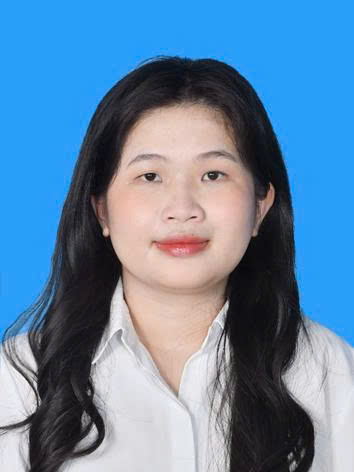
\includegraphics[
        width=2.2cm,
        height=2.7cm,
        keepaspectratio
    ]{assets/avt.jpg}
\end{minipage}

\end{tabularx}

\vspace{3pt}
\textcolor{rulecol}{\rule{\linewidth}{0.6pt}}

% ─── CAREER OBJECTIVE ─────────────────────────────────
\section*{Career Objective}

{\small
Final-year Information Technology student seeking a Software Developer
position, with hands-on experience in Python, TypeScript/JavaScript, and
Kotlin, building backend services and RESTful APIs (FastAPI, Node.js, NestJS),
event-driven systems with Kafka and RabbitMQ, and database-driven
applications. Experienced in team projects using Git, Docker, Jira, and
Confluence, and in integrating AI models into full applications. Eager to
write clean, maintainable code and grow as a developer.
}

% ─── EDUCATION ────────────────────────────────────────
\section*{Education}

\entry
{University of Transport Ho Chi Minh City (UTH)}
{10/2022 -- 10/2026}
{Bachelor of Information Technology -- Completed coursework}

{\small
\begin{cvitems}
    \item GPA: 3.4 / 4.0
    \item \textbf{Excellent Scholarship} -- Semester 1, 2025
    \item \textbf{Second Prize -- AI Track},
    UTH Student Scientific Research Conference 2025
\end{cvitems}
}

% ─── TECHNICAL SKILLS ─────────────────────────────────
\section*{Technical Skills}

{\small
\begin{tabularx}{\linewidth}{@{}lX@{}}

\textbf{Programming}
&
Python, TypeScript, JavaScript, Kotlin, SQL
\\[1pt]

\textbf{Backend / API}
&
FastAPI, Node.js, NestJS, RESTful API, Microservices, Postman
\\[1pt]

\textbf{Messaging / Architecture}
&
Apache Kafka, RabbitMQ, Event-driven Architecture, MinIO
\\[1pt]

\textbf{Databases}
&
PostgreSQL, SQL Server, MySQL, MongoDB, Firebase, Supabase
\\[1pt]

\textbf{Frontend / Mobile}
&
Next.js, Kotlin (Android)
\\[1pt]

\textbf{AI Integration}
&
PyTorch, YOLO, Transformer, LLMs, RAG
\\[1pt]

\textbf{Data / Automation}
&
ETL/ELT, dbt, Apache Airflow, Power BI
\\[1pt]

\textbf{DevOps / Tools}
&
Git, Docker, Jira, Confluence, VS Code

\end{tabularx}
}

% ─── WORK EXPERIENCE ──────────────────────────────────
\section*{Work Experience}

\entry
{Gotik Consulting -- Data Engineer}
{Python \textbar{} dbt \textbar{} PostgreSQL \textbar{} Airflow \textbar{} Power BI}
{03/2026 -- 05/2026}

{\small
\begin{cvitems}

    \item Wrote Python scripts and ETL pipelines to extract, clean, transform, and load Odoo business data into Neon PostgreSQL.

    \item Developed dbt models and SQL queries to turn raw data into structured, reusable datasets that are easy to maintain.

    \item Automated hourly workflows with Apache Airflow, including task scheduling, dependency management, and monitoring of runs.

    \item Built Power BI dashboards for operational monitoring and data-driven insights.

\end{cvitems}
}

% ─── PROJECTS ─────────────────────────────────────────
\section*{Featured Projects}

\entry
{Fall Detection -- Real-Time AI Fall Detection System}
{Python \textbar{} YOLOv8 Pose \textbar{} MediaPipe \textbar{} Transformer \textbar{} FastAPI}
{04/2026 -- 06/2026}

{\small
\begin{cvitems}
    \item Developed a real-time fall detection system using YOLOv8 Pose, MediaPipe, and Transformer.
    \item Trained a Transformer Encoder with 30-frame $\times$ 200-feature input for fall/non-fall classification.
    \item Achieved 97.8\% mean accuracy with 5-fold cross-validation and integrated FastAPI for real-time alerts.
    \item GitHub: \href{https://github.com/hohuynhnhu/Fall-Detection}{Fall-Detection}
\end{cvitems}
}

\vspace{3pt}

\entry
{VehicleScan -- Smart Parking System with AI \& IoT}
{Python \textbar{} YOLO \textbar{} CNN \textbar{} Siamese Network \textbar{} ESP32}
{03/2025 -- 03/2026}

{\small
\begin{cvitems}
    \item Developed vehicle detection and recognition models using YOLO, CNN, and Siamese Network.
    \item Prepared datasets and trained AI models for real-time vehicle identification.
    \item Integrated AI models with ESP32 and Firebase; won Second Prize -- AI Track at UTH 2025.
    \item GitHub: \href{https://github.com/LeKhang-cn22h/VehicleScanner.git}{VehicleScanner}
\end{cvitems}
}


\vspace{3pt}

\entry
{Delivery Driver -- Order Management \& Data Analytics System}
{Python \textbar{} PostgreSQL \textbar{} Kafka \textbar{} MinIO \textbar{} RFM \textbar{} Association Rule Mining}
{12/2025 -- 02/2026}

{\small

\begin{cvitems}
    \item Built an automated, event-based data pipeline with Kafka, a MinIO Data Lake, and a PostgreSQL Data Warehouse to ingest and process order data in real time.
    \item Applied RFM and Association Rule Mining (Python) to analyze customer orders and frequent pickup--delivery location pairs.
    \item Generated location-based insights to support recommendations for opening new post offices or service locations.
    \item GitHub: \href{https://github.com/LeKhang-cn22h/BE-delivery-driver}{BE-delivery-driver}
\end{cvitems}

}

% % ─── ADDITIONAL INFORMATION ───────────────────────────
% \section*{Additional Information}

% {\small
% \begin{tabularx}{\linewidth}{@{}lX@{}}

% \textbf{Soft Skills}
% &
% Problem-solving \textbar{}
% Troubleshooting \textbar{}
% Teamwork \textbar{}
% Research and self-learning
% \\[2pt]

% \textbf{English}
% &
% Technical document reading and basic professional communication
% \\[2pt]

% \textbf{Availability}
% &
% Available for full-time Software Developer opportunities.

% \end{tabularx}
% }

\end{document}